% 1977 年青海卷第三题：长方体 ABCD-A'B'C'D'（顶面 A'B'C'D'），底面 ABCD（A 前左、B 前右、
% C 后右、D 后左），体对角线 AC' 与 A'C 交于体心 O，∠AOC=120°，辅助线底面对角线 AC（虚线）
%（按源卷第 1 页布局）
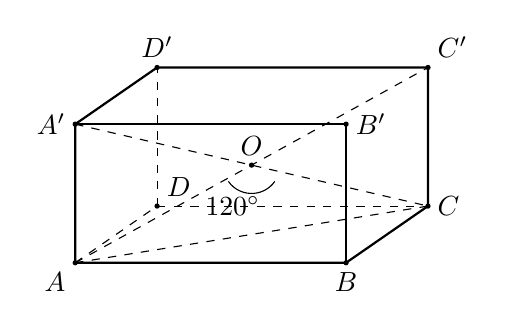
\begin{tikzpicture}[scale=0.8]
  \coordinate (A) at (0,0);
  \coordinate (B) at (4.3,0);
  \coordinate (C) at (5.6,0.9);
  \coordinate (D) at (1.3,0.9);
  \coordinate (A1) at (0,2.2);
  \coordinate (B1) at (4.3,2.2);
  \coordinate (C1) at (5.6,3.1);
  \coordinate (D1) at (1.3,3.1);
  \coordinate (O) at (2.8,1.55);
  \draw[thick] (A)--(B)--(C)--(C1)--(D1)--(A1)--cycle;
  \draw[thick] (A)--(A1);
  \draw[thick] (B)--(B1);
  \draw[thick] (A1)--(B1);
  \draw[dashed] (A)--(D);
  \draw[dashed] (D)--(C);
  \draw[dashed] (D)--(D1);
  \draw[dashed] (A)--(C);
  \draw[dashed] (A)--(C1);
  \draw[dashed] (A1)--(C);
  \fill (A) circle (1.2pt) node[below left] {$A$};
  \fill (B) circle (1.2pt) node[below] {$B$};
  \fill (C) circle (1.2pt) node[right] {$C$};
  \fill (D) circle (1.2pt) node[above right] {$D$};
  \fill (A1) circle (1.2pt) node[left] {$A'$};
  \fill (B1) circle (1.2pt) node[right] {$B'$};
  \fill (C1) circle (1.2pt) node[above right] {$C'$};
  \fill (D1) circle (1.2pt) node[above] {$D'$};
  \fill (O) circle (1.2pt) node[above] {$O$};
  \draw ([shift={(215:0.45)}]O) arc[start angle=215, end angle=325, radius=0.45];
  \node at (2.5,0.9) {$120^\circ$};
\end{tikzpicture}
